\documentclass[12pt, a4paper]{article}

%% ── Geometry ────────────────────────────────────────────────────────────────
\usepackage[a4paper, top=2.5cm, bottom=2.5cm,
            left=2.8cm, right=2.8cm, headheight=15pt]{geometry}

%% ── Fonts & encoding ────────────────────────────────────────────────────────
\usepackage[T1]{fontenc}
\usepackage[utf8]{inputenc}
\usepackage{palatino}
\usepackage{mathpazo}
\usepackage{microtype}

%% ── Mathematics ─────────────────────────────────────────────────────────────
\usepackage{amsmath, amssymb, amsthm, mathtools}
\usepackage{cancel}

%% ── Graphics & colour ───────────────────────────────────────────────────────
\usepackage{xcolor}
\usepackage{tikz}
\usetikzlibrary{arrows.meta, positioning, calc,
                decorations.pathreplacing, backgrounds, patterns}
\usepackage{pgfplots}
\pgfplotsset{compat=1.15}

%% ── Tables ──────────────────────────────────────────────────────────────────
\usepackage{booktabs, array, colortbl, multirow, tabularx}
\renewcommand{\arraystretch}{1.45}

%% ── Lists ───────────────────────────────────────────────────────────────────
\usepackage{enumitem}
\setlist[itemize]{leftmargin=1.8em, itemsep=3pt, topsep=4pt}
\setlist[enumerate]{leftmargin=1.8em, itemsep=3pt, topsep=4pt}

%% ── Callout boxes ───────────────────────────────────────────────────────────
\usepackage[most]{tcolorbox}
\tcbuselibrary{skins, breakable, theorems}

%% ── Headers, footers, TOC, captions ────────────────────────────────────────
\usepackage{fancyhdr}
\usepackage{lastpage}
\usepackage{tocloft}
\usepackage{caption}
\usepackage{float}

%% ── Hyperlinks ──────────────────────────────────────────────────────────────
\usepackage[colorlinks=true, linkcolor=indigo,
            urlcolor=indigo, citecolor=indigo]{hyperref}

%% ── Spacing ─────────────────────────────────────────────────────────────────
\usepackage{parskip}
\setlength{\parskip}{6pt}
\setlength{\parindent}{0pt}

%% ═══════════════════════════════════════════════════════════════════════════
%%  COLOUR PALETTE  (deep indigo / amber / teal / crimson)
%% ═══════════════════════════════════════════════════════════════════════════
\definecolor{indigo}{RGB}{48, 28, 120}
\definecolor{indigolight}{RGB}{234, 230, 252}
\definecolor{amber}{RGB}{178, 120, 6}
\definecolor{lightamber}{RGB}{255, 248, 215}
\definecolor{teal}{RGB}{8, 108, 98}
\definecolor{lightteal}{RGB}{222, 248, 243}
\definecolor{crimson}{RGB}{148, 18, 28}
\definecolor{lightcrimson}{RGB}{255, 234, 234}
\definecolor{purple}{RGB}{90, 28, 145}
\definecolor{lightpurple}{RGB}{245, 237, 255}
\definecolor{solgreen}{RGB}{8, 92, 48}
\definecolor{lightsol}{RGB}{225, 252, 236}
\definecolor{charcoal}{RGB}{36, 36, 36}
\definecolor{slate}{RGB}{72, 84, 100}
\definecolor{tabhead}{RGB}{48, 28, 120}
\definecolor{tabeven}{RGB}{234, 230, 252}
\definecolor{orange}{RGB}{195, 90, 10}
\definecolor{lightorange}{RGB}{255, 242, 225}
\definecolor{forestgreen}{RGB}{22, 100, 42}
\definecolor{lightforest}{RGB}{228, 248, 232}

%% ═══════════════════════════════════════════════════════════════════════════
%%  TCOLORBOX ENVIRONMENTS
%% ═══════════════════════════════════════════════════════════════════════════
\newtcolorbox{defbox}[1]{breakable, enhanced,
  colback=indigolight, colframe=indigo, coltitle=white,
  fonttitle=\bfseries\sffamily, title={Definition\quad#1},
  arc=4pt, boxrule=1pt, left=8pt, right=8pt, top=6pt, bottom=6pt,
  attach boxed title to top left={yshift=-2mm, xshift=6mm},
  boxed title style={colback=indigo, arc=3pt, boxrule=0pt}}

\newtcolorbox{thmbox}[1]{breakable, enhanced,
  colback=lightteal, colframe=teal, coltitle=white,
  fonttitle=\bfseries\sffamily, title={Theorem\quad#1},
  arc=4pt, boxrule=1pt, left=8pt, right=8pt, top=6pt, bottom=6pt,
  attach boxed title to top left={yshift=-2mm, xshift=6mm},
  boxed title style={colback=teal, arc=3pt, boxrule=0pt}}

\newtcolorbox{propbox}[1]{breakable, enhanced,
  colback=lightteal, colframe=teal, coltitle=white,
  fonttitle=\bfseries\sffamily, title={Proposition\quad#1},
  arc=4pt, boxrule=1pt, left=8pt, right=8pt, top=6pt, bottom=6pt,
  attach boxed title to top left={yshift=-2mm, xshift=6mm},
  boxed title style={colback=teal, arc=3pt, boxrule=0pt}}

\newtcolorbox{keybox}[1]{breakable, enhanced,
  colback=lightamber, colframe=amber, coltitle=white,
  fonttitle=\bfseries\sffamily, title={#1},
  arc=4pt, boxrule=1pt, left=8pt, right=8pt, top=6pt, bottom=6pt,
  attach boxed title to top left={yshift=-2mm, xshift=6mm},
  boxed title style={colback=amber, arc=3pt, boxrule=0pt}}

\newtcolorbox{exbox}[1]{breakable, enhanced,
  colback=lightpurple, colframe=purple, coltitle=white,
  fonttitle=\bfseries\sffamily, title={Worked Example\quad#1},
  arc=4pt, boxrule=1pt, left=8pt, right=8pt, top=6pt, bottom=6pt,
  attach boxed title to top left={yshift=-2mm, xshift=6mm},
  boxed title style={colback=purple, arc=3pt, boxrule=0pt}}

\newtcolorbox{warnbox}[1]{breakable, enhanced,
  colback=lightcrimson, colframe=crimson, coltitle=white,
  fonttitle=\bfseries\sffamily, title={#1},
  arc=4pt, boxrule=1pt, left=8pt, right=8pt, top=6pt, bottom=6pt,
  attach boxed title to top left={yshift=-2mm, xshift=6mm},
  boxed title style={colback=crimson, arc=3pt, boxrule=0pt}}

\newtcolorbox{notebox}[1]{breakable, enhanced,
  colback=lightorange, colframe=orange, coltitle=white,
  fonttitle=\bfseries\sffamily, title={#1},
  arc=4pt, boxrule=1pt, left=8pt, right=8pt, top=6pt, bottom=6pt,
  attach boxed title to top left={yshift=-2mm, xshift=6mm},
  boxed title style={colback=orange, arc=3pt, boxrule=0pt}}

\newtcolorbox{factbox}[1]{breakable, enhanced,
  colback=lightforest, colframe=forestgreen, coltitle=white,
  fonttitle=\bfseries\sffamily, title={#1},
  arc=4pt, boxrule=1pt, left=8pt, right=8pt, top=6pt, bottom=6pt,
  attach boxed title to top left={yshift=-2mm, xshift=6mm},
  boxed title style={colback=forestgreen, arc=3pt, boxrule=0pt}}

\newtcolorbox{solbox}{breakable, enhanced,
  colback=lightsol, colframe=solgreen, coltitle=white,
  fonttitle=\bfseries\sffamily, title={Solution},
  arc=4pt, boxrule=1pt, left=8pt, right=8pt, top=6pt, bottom=6pt,
  attach boxed title to top left={yshift=-2mm, xshift=6mm},
  boxed title style={colback=solgreen, arc=3pt, boxrule=0pt}}

%% ── Theorem-style environments ──────────────────────────────────────────────
\theoremstyle{definition}
\newtheorem{remark}{Remark}[section]

%% ═══════════════════════════════════════════════════════════════════════════
%%  MATHS MACROS
%% ═══════════════════════════════════════════════════════════════════════════
\newcommand{\R}{\mathbb{R}}
\newcommand{\N}{\mathbb{N}}
\newcommand{\Z}{\mathbb{Z}}
\newcommand{\e}{\mathrm{e}}
\newcommand{\dd}[1]{\,d#1}
\newcommand{\ddd}[2]{\dfrac{d#1}{d#2}}
\newcommand{\dddd}[2]{\dfrac{d^{2}#1}{d#2^{2}}}
\newcommand{\pp}[2]{\dfrac{\partial #1}{\partial #2}}
\newcommand{\eval}[2]{\left.#1\right|_{#2}}
\newcommand{\abs}[1]{\left|#1\right|}
\newcommand{\limit}[2]{\lim_{#1 \to #2}}
\newcommand{\bx}{\mathbf{x}}
\DeclareMathOperator{\sgn}{sgn}

%% ═══════════════════════════════════════════════════════════════════════════
%%  PAGE STYLE
%% ═══════════════════════════════════════════════════════════════════════════
\pagestyle{fancy}
\fancyhf{}
\fancyhead[L]{\textcolor{indigo}{\textbf{ECON 320}}
  \textcolor{slate}{ --- Exponential and Logarithmic Functions}}
\fancyhead[R]{\textcolor{slate}{\small Chiang \& Wainwright (2005), Ch.\ 10}}
\fancyfoot[C]{\textcolor{slate}{\small Page \thepage\ of \pageref{LastPage}}}
\renewcommand{\headrulewidth}{1.2pt}
\renewcommand{\headrule}{%
  \hbox to\headwidth{\color{indigo}\leaders\hrule height\headrulewidth\hfill}}
\renewcommand{\footrulewidth}{0.4pt}

\renewcommand{\cftsecfont}{\bfseries\color{indigo}}
\renewcommand{\cftsecpagefont}{\bfseries\color{indigo}}
\renewcommand{\cftsubsecfont}{\color{charcoal}}
\setlength{\cftbeforesecskip}{4pt}

%% ═══════════════════════════════════════════════════════════════════════════
\begin{document}
%% ═══════════════════════════════════════════════════════════════════════════

%% ── COVER ───────────────────────────────────────────────────────────────────
\thispagestyle{empty}
\begin{tikzpicture}[remember picture, overlay]
  \fill[indigo] (current page.north west)
    rectangle ([yshift=-6.2cm] current page.north east);
  \fill[amber]  ([yshift=-6.2cm] current page.north west)
    rectangle ([yshift=-6.65cm] current page.north east);
\end{tikzpicture}

\vspace*{-1.7cm}
\begin{center}
  {\color{white}\large\bfseries\sffamily ECON 320 --- LECTURE NOTES}\\[10pt]
  {\color{white}\Huge\bfseries Exponential and}\\[6pt]
  {\color{white}\Huge\bfseries Logarithmic Functions}\\[10pt]
  {\color{amber}\large\itshape
   Chiang \& Wainwright (2005) Ch.\ 10\quad|\quad
   Hoy et al.\ (2011)\quad|\quad Simon \& Blume (1994)}
\end{center}

\vspace{3.8cm}
\begin{center}
\begin{tabular}{r l}
  \textbf{\textcolor{indigo}{Course}}
    & ECON 320: Mathematical Economics III \\[3pt]
  \textbf{\textcolor{indigo}{Primary Text}}
    & A.\ C.\ Chiang \& K.\ Wainwright,
      \textit{Fundamental Methods of Mathematical Economics},\\
    & 4th ed., McGraw-Hill, 2005. Ch.\ 10. \\[3pt]
  \textbf{\textcolor{indigo}{Supplementary}}
    & Hoy, Livernois, McKenna, Rees \& Stengos,
      \textit{Mathematics for Economics},\\
    & 3rd ed., MIT Press, 2011. Ch.\ 6. \\[2pt]
    & Simon \& Blume,
      \textit{Mathematics for Economists}, Norton, 1994. Ch.\ 25. \\[3pt]
  \textbf{\textcolor{indigo}{Topics}}
    & Exponential functions, the number $\e$, logarithmic functions,\\
    & laws of exponents and logarithms, natural logarithm,\\
    & differentiation and integration, economic applications:\\
    & compound interest, continuous growth, elasticity, log-linearisation. \\[3pt]
  \textbf{\textcolor{indigo}{Date}} & May 2026 \\
\end{tabular}
\end{center}

\newpage
\tableofcontents
\newpage

%% ═══════════════════════════════════════════════════════════════════════════
\section{Introduction: Why Exponential and Log Functions in Economics?}
%% ═══════════════════════════════════════════════════════════════════════════

Exponential and logarithmic functions are indispensable in economic analysis. Their ubiquity stems from a single, fundamental observation: \emph{many economic quantities grow (or decay) at a rate proportional to their current level}. When a quantity's rate of change is proportional to the quantity itself, the law of motion is an exponential function. Examples include:

\begin{itemize}
  \item \textbf{Capital accumulation}: $\dot K = sY$ leads to exponential growth paths in neoclassical growth models.
  \item \textbf{Compound interest}: A principal $P$ at rate $r$ grows as $P(1+r)^t$, approaching $Pe^{rt}$ under continuous compounding.
  \item \textbf{Price dynamics}: Inflation at a constant rate $\pi$ implies price level $P_t = P_0 e^{\pi t}$.
  \item \textbf{Discounting}: The present value of a future payment uses $e^{-rt}$ under continuous discounting.
  \item \textbf{Econometrics}: Log-linear specifications yield constant elasticities, simplify multiplicative models, and appear in almost every estimated demand and production equation.
\end{itemize}

Moreover, the natural logarithm transforms multiplicative relationships into additive ones, converts power functions into linear ones, and provides the cleanest measure of proportional change. For an economist, $\ln$ is as essential a tool as the derivative itself.

%% ═══════════════════════════════════════════════════════════════════════════
\section{Exponential Functions}
%% ═══════════════════════════════════════════════════════════════════════════

\subsection{Definition and Basic Properties}

\begin{defbox}{Exponential Function}
An \textbf{exponential function} has the form:
\[
  f(x) = b^x, \qquad b > 0,\; b \neq 1,\; x \in \R
\]
where $b$ is the \textbf{base} and $x$ is the \textbf{exponent}. The domain is all of $\R$ and the range is $(0, \infty)$.
\end{defbox}

The behaviour depends critically on the base:
\begin{itemize}
  \item $b > 1$: $f(x) = b^x$ is \textbf{strictly increasing} (exponential growth). As $x \to \infty$, $f(x) \to \infty$; as $x \to -\infty$, $f(x) \to 0$.
  \item $0 < b < 1$: $f(x) = b^x$ is \textbf{strictly decreasing} (exponential decay). As $x \to \infty$, $f(x) \to 0$; as $x \to -\infty$, $f(x) \to \infty$.
  \item In all cases: $f(0) = b^0 = 1$, so every exponential function passes through $(0,1)$.
\end{itemize}

\begin{center}
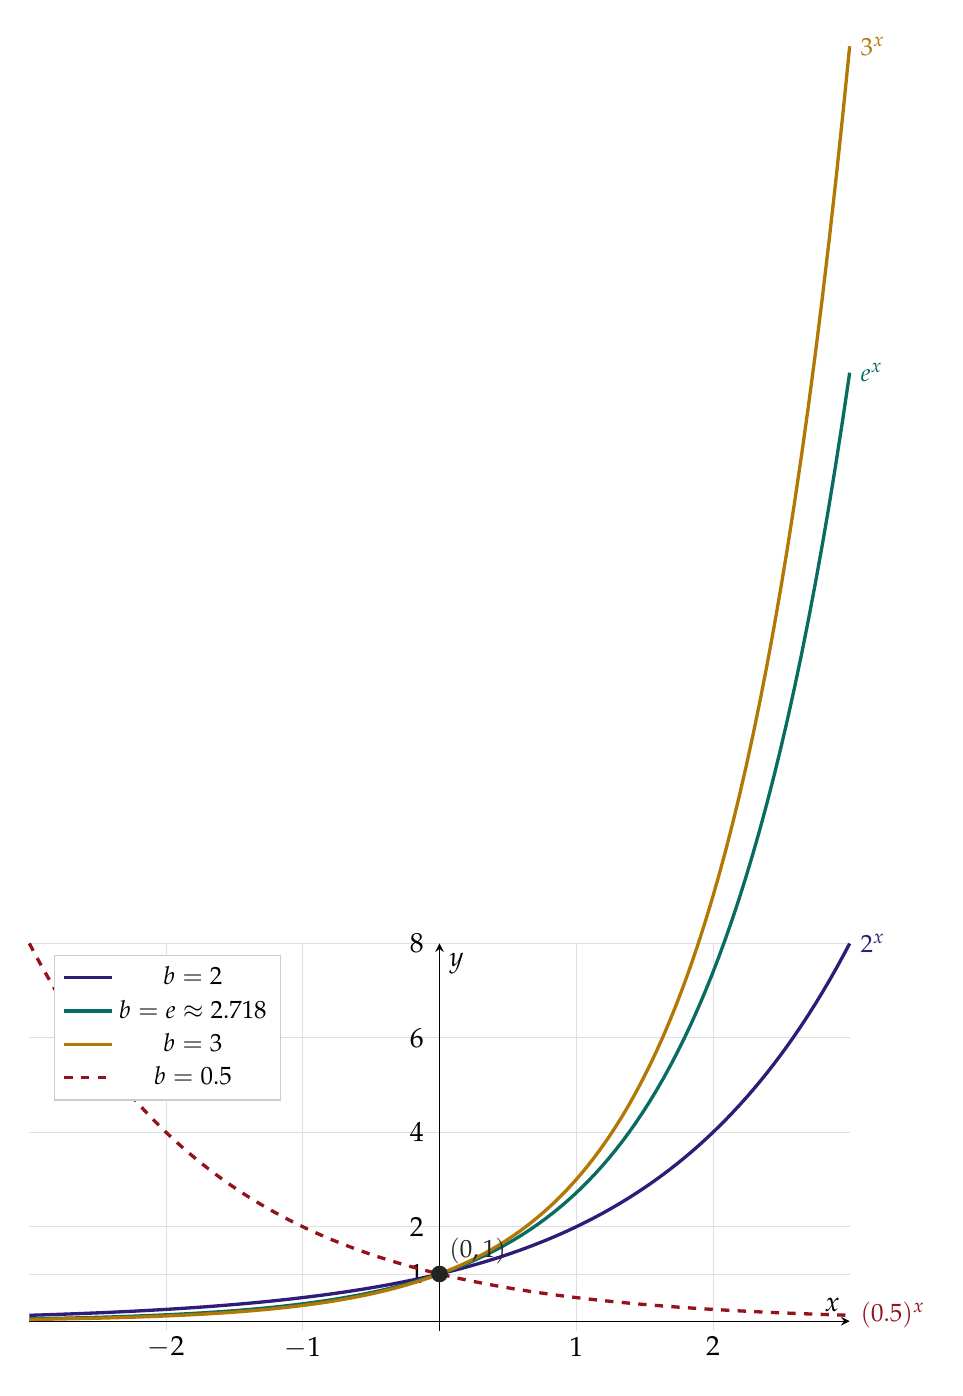
\begin{tikzpicture}
\begin{axis}[
  width=12cm, height=6.5cm,
  axis lines=center,
  xlabel={$x$}, ylabel={$y$},
  xmin=-3, xmax=3, ymin=-0.2, ymax=8,
  xtick={-2,-1,0,1,2},
  ytick={1,2,4,6,8},
  tick style={draw=none},
  grid=both, grid style={line width=0.3pt, draw=gray!25},
  legend pos=north west,
  legend style={font=\small, draw=gray!40},
  clip=false,
]
  \addplot[indigo, very thick, domain=-3:3, samples=120]{2^x}
    node[right, pos=1, font=\small]{$2^x$};
  \addplot[teal, very thick, domain=-3:3, samples=120]{exp(x)}
    node[right, pos=1, font=\small]{$e^x$};
  \addplot[amber, very thick, domain=-3:3, samples=120]{3^x}
    node[right, pos=1, font=\small]{$3^x$};
  \addplot[crimson, very thick, dashed, domain=-3:3, samples=120]{0.5^x}
    node[right, pos=1, font=\small]{$(0.5)^x$};
  \addplot[only marks, mark=*, mark size=2.8pt, charcoal]
    coordinates{(0,1)};
  \node[charcoal, above right, font=\small] at (axis cs:0,1){$(0,1)$};
  \addlegendentry{$b=2$}
  \addlegendentry{$b=e\approx 2.718$}
  \addlegendentry{$b=3$}
  \addlegendentry{$b=0.5$}
\end{axis}
\end{tikzpicture}
\captionof*{figure}{\small All exponential functions pass through $(0,1)$. Larger bases grow faster; bases less than 1 decay. The natural base $e$ occupies a special position.}
\end{center}

\subsection{Laws of Exponents}

\begin{thmbox}{Laws of Exponents}
For $b > 0$, $c > 0$, and all $x, y \in \R$:
\begin{center}
\begin{tabular}{lll}
  \toprule
  \rowcolor{tabhead}
  \color{white}\textbf{Law} & \color{white}\textbf{Statement} & \color{white}\textbf{Example} \\
  \midrule
  Product rule & $b^x \cdot b^y = b^{x+y}$ & $2^3 \cdot 2^4 = 2^7 = 128$ \\
  \rowcolor{tabeven}
  Quotient rule & $b^x / b^y = b^{x-y}$ & $5^6 / 5^2 = 5^4 = 625$ \\
  Power rule & $(b^x)^y = b^{xy}$ & $(3^2)^4 = 3^8 = 6561$ \\
  \rowcolor{tabeven}
  Base product & $(bc)^x = b^x c^x$ & $(2 \cdot 3)^4 = 2^4 \cdot 3^4 = 1296$ \\
  Base quotient & $(b/c)^x = b^x / c^x$ & $(4/2)^3 = 4^3/2^3 = 8$ \\
  \rowcolor{tabeven}
  Zero exponent & $b^0 = 1$ & $7^0 = 1$ \\
  Negative exponent & $b^{-x} = 1/b^x$ & $2^{-3} = 1/8$ \\
  \rowcolor{tabeven}
  Fractional exponent & $b^{p/q} = (b^{1/q})^p = \sqrt[q]{b^p}$ & $8^{2/3} = (\sqrt[3]{8})^2 = 4$ \\
  \bottomrule
\end{tabular}
\end{center}
\emph{(Chiang \& Wainwright, p.\ 268; Simon \& Blume, Ch.\ 25)}
\end{thmbox}

\begin{exbox}{Simplifying Exponential Expressions}
\textbf{1.} Simplify $\dfrac{(2x^3)^4 \cdot x^{-2}}{8x^5}$:
\[
  \frac{16x^{12} \cdot x^{-2}}{8x^5}
  = \frac{16x^{10}}{8x^5}
  = 2x^5
\]

\textbf{2.} Solve for $x$: $4^x = 8$.
\[
  (2^2)^x = 2^3 \implies 2^{2x} = 2^3 \implies 2x = 3 \implies x = \frac{3}{2}
\]

\textbf{3.} In economics, the Cobb-Douglas production function
$Y = AK^\alpha L^\beta$ uses fractional exponents. Here $K^{0.3}$ means
$K^{3/10} = \sqrt[10]{K^3}$, and the law $(tK)^\alpha(tL)^\beta = t^{\alpha+\beta}K^\alpha L^\beta$ follows directly from the base-product rule.
\end{exbox}

\subsection{The Number $e$ and the Natural Exponential}

The most important base in mathematics and economics is the irrational number $e \approx 2.71828\ldots$, known as \textbf{Euler's number}.

\begin{defbox}{The Number $e$}
The number $e$ is defined as:
\[
  e = \lim_{n \to \infty}\left(1 + \frac{1}{n}\right)^n
    = \lim_{h \to 0}(1 + h)^{1/h}
    \approx 2.71828182845\ldots
\]
It also equals the sum of the series:
\[
  e = \sum_{n=0}^{\infty} \frac{1}{n!}
    = 1 + 1 + \frac{1}{2} + \frac{1}{6} + \frac{1}{24} + \cdots
\]
The function $f(x) = e^x$ is called the \textbf{natural exponential function}.
\end{defbox}

\begin{keybox}{Why is $e$ Special?}
The number $e$ is the unique base for which:
\begin{enumerate}
  \item $\dfrac{d}{dx}[e^x] = e^x$ --- the natural exponential is its own derivative.
  \item $\displaystyle\int e^x \dd{x} = e^x + C$.
  \item The tangent line to $y = e^x$ at $(0,1)$ has slope exactly 1.
  \item The solution to $\dot y = ky$ (proportional growth) is $y(t) = y_0 e^{kt}$.
\end{enumerate}
No other base has property (1), which makes $e$ the ``natural'' choice for
calculus and differential equations. \emph{(Chiang \& Wainwright, p.\ 271)}
\end{keybox}

\begin{exbox}{Deriving $e$ from Compound Interest}
A bank offers annual interest rate $r$. If interest is compounded $n$ times per year, \$1 invested grows to $\left(1 + \dfrac{r}{n}\right)^n$ after one year.

\begin{center}
\begin{tabular}{lll}
  \toprule
  \rowcolor{tabhead}
  \color{white}$n$ (compoundings/yr) & \color{white}Formula & \color{white}Value at $r=1$ (100\%) \\
  \midrule
  1 (annual) & $(1+1)^1$ & $2.000$ \\
  \rowcolor{tabeven}
  2 (semi-annual) & $(1+0.5)^2$ & $2.250$ \\
  4 (quarterly) & $(1+0.25)^4$ & $2.441$ \\
  \rowcolor{tabeven}
  12 (monthly) & $(1+1/12)^{12}$ & $2.613$ \\
  365 (daily) & $(1+1/365)^{365}$ & $2.715$ \\
  \rowcolor{tabeven}
  $\infty$ (continuous) & $\lim_{n\to\infty}(1+1/n)^n$ & $e = 2.718\ldots$ \\
  \bottomrule
\end{tabular}
\end{center}

As $n \to \infty$, the limit is $e^r$. \textbf{Under continuous compounding at rate $r$}, \$1 grows to $e^r$ in one year and to $e^{rt}$ in $t$ years.

This derivation shows that $e$ emerges naturally from the mathematics of interest, making it the canonical base for financial and economic modelling.
\end{exbox}

%% ═══════════════════════════════════════════════════════════════════════════
\section{Logarithmic Functions}
%% ═══════════════════════════════════════════════════════════════════════════

\subsection{Definition as the Inverse of the Exponential}

\begin{defbox}{Logarithm}
The \textbf{logarithm base $b$} of a positive number $y$ is the exponent $x$ such that $b^x = y$:
\[
  x = \log_b y \iff b^x = y, \qquad b > 0,\; b \neq 1,\; y > 0
\]
The logarithm is the \textbf{inverse function} of the exponential:
$\log_b(b^x) = x$ for all $x \in \R$, and $b^{\log_b y} = y$ for all $y > 0$.

The domain of $\log_b$ is $(0, \infty)$ and the range is $\R$.
\end{defbox}

\begin{defbox}{Natural Logarithm}
The \textbf{natural logarithm} is the logarithm base $e$:
\[
  \ln y = \log_e y \iff e^x = y
\]
It is the inverse of the natural exponential: $\ln(e^x) = x$ and $e^{\ln y} = y$.

The natural log is the standard logarithm in economics and calculus because of its clean derivative and integral properties. \emph{(Chiang \& Wainwright, p.\ 275)}
\end{defbox}

\begin{center}
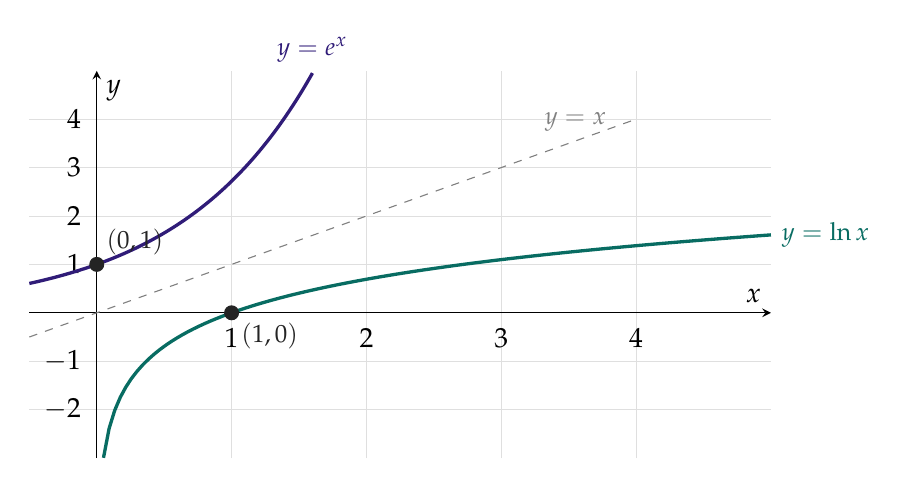
\begin{tikzpicture}
\begin{axis}[
  width=11cm, height=6.5cm,
  axis lines=center,
  xlabel={$x$}, ylabel={$y$},
  xmin=-0.5, xmax=5, ymin=-3, ymax=5,
  xtick={1,2,3,4},
  ytick={-2,-1,0,1,2,3,4},
  tick style={draw=none},
  grid=both, grid style={line width=0.3pt, draw=gray!25},
  clip=false,
]
  %% e^x
  \addplot[indigo, very thick, domain=-0.5:1.6, samples=100]{exp(x)}
    node[above, pos=1, font=\small, indigo]{$y=e^x$};
  %% ln x
  \addplot[teal, very thick, domain=0.05:5, samples=120]{ln(x)}
    node[right, pos=1, font=\small, teal]{$y=\ln x$};
  %% Mirror line y=x
  \addplot[gray, dashed, domain=-0.5:4, samples=2]{x}
    node[above, pos=0.9, font=\small, gray]{$y=x$};
  %% Key points
  \addplot[only marks, mark=*, mark size=2.5pt, charcoal]
    coordinates{(0,1)(1,0)};
  \node[charcoal, above right, font=\small] at (axis cs:0,1){$(0,1)$};
  \node[charcoal, below right, font=\small] at (axis cs:1,0){$(1,0)$};
\end{axis}
\end{tikzpicture}
\captionof*{figure}{\small $y=e^x$ and $y=\ln x$ are reflections of each other across the line $y=x$, confirming they are inverse functions. Note $e^0=1\Leftrightarrow \ln 1=0$; $e^1=e\Leftrightarrow \ln e=1$.}
\end{center}

\subsection{Laws of Logarithms}

\begin{thmbox}{Laws of Logarithms}
For $b>0$, $b\neq 1$, and positive numbers $M$, $N$:
\[
  \log_b(MN) = \log_b M + \log_b N \tag{Product}
\]
\[
  \log_b\!\left(\frac{M}{N}\right) = \log_b M - \log_b N \tag{Quotient}
\]
\[
  \log_b(M^p) = p\,\log_b M, \quad p \in \R \tag{Power}
\]
\[
  \log_b b = 1 \tag{Base}
\]
\[
  \log_b 1 = 0 \tag{Unity}
\]
\[
  \log_b M = \frac{\ln M}{\ln b} = \frac{\log_a M}{\log_a b} \tag{Change of Base}
\]
In particular, writing these for the natural log ($b = e$):
\[
  \ln(MN)=\ln M+\ln N,\quad
  \ln\!\left(\frac{M}{N}\right)=\ln M-\ln N,\quad
  \ln(M^p)=p\ln M
\]
\end{thmbox}

\begin{proof}[Proof of the Product Law]
Let $x = \log_b M$ and $y = \log_b N$, so $M = b^x$ and $N = b^y$.
Then $MN = b^x \cdot b^y = b^{x+y}$ by the product rule for exponents.
Therefore $\log_b(MN) = x+y = \log_b M + \log_b N$. \qed
\end{proof}

\begin{exbox}{Applying the Laws of Logarithms}
\textbf{1.} Expand $\ln\!\left(\dfrac{x^2\sqrt{y}}{z^3}\right)$:
\[
  \ln\!\left(\frac{x^2 y^{1/2}}{z^3}\right)
  = \ln(x^2) + \ln(y^{1/2}) - \ln(z^3)
  = 2\ln x + \tfrac{1}{2}\ln y - 3\ln z
\]

\textbf{2.} Solve $2\ln x + \ln(x+1) = \ln 12$:
\[
  \ln(x^2) + \ln(x+1) = \ln 12
  \implies \ln[x^2(x+1)] = \ln 12
  \implies x^2(x+1) = 12
  \implies x^3 + x^2 - 12 = 0
\]
Factor: $(x-2)(x^2+3x+6)=0$. Check: $x^3+x^2-12$ at $x=2$: $8+4-12=0$. \checkmark

So $x=2$ (the quadratic $x^2+3x+6$ has no real roots since discriminant $=9-24<0$).

\textbf{3. Log-linearising Cobb-Douglas:}
$Y = AK^\alpha L^\beta$. Taking logs:
\[
  \ln Y = \ln A + \alpha \ln K + \beta \ln L
\]
This converts the multiplicative model into a linear one, enabling OLS regression. The coefficient $\alpha$ is directly the elasticity of output with respect to capital, and $\beta$ is the labour elasticity.

\textbf{4.} Change of base: $\log_8 32$.
\[
  \log_8 32 = \frac{\ln 32}{\ln 8} = \frac{\ln 2^5}{\ln 2^3} = \frac{5\ln 2}{3\ln 2} = \frac{5}{3}
\]
\end{exbox}

\subsection{Relationship Between $e$ and $\ln$}

\begin{factbox}{Key Identities: $e$ and $\ln$}
\begin{align*}
  \ln e &= 1 & e^0 &= 1 \Rightarrow \ln 1 = 0 \\
  \ln(e^x) &= x \quad \forall x \in \R & e^{\ln y} &= y \quad \forall y > 0 \\
  \ln e^r &= r & e^{\ln a + \ln b} &= ab \\
  \ln(1+r) &\approx r \text{ for small } r & e^r &\approx 1+r \text{ for small } r
\end{align*}
The approximations $\ln(1+r)\approx r$ and $e^r\approx 1+r$ are widely used
for small growth rates $r$ (e.g.\ quarterly inflation or interest rates).
\end{factbox}

%% ═══════════════════════════════════════════════════════════════════════════
\section{Differentiation of Exponential and Logarithmic Functions}
%% ═══════════════════════════════════════════════════════════════════════════

\subsection{Derivatives of Exponential Functions}

\begin{thmbox}{Derivatives of Exponential Functions}
\begin{align}
  \ddd{}{x}[e^x] &= e^x \label{eq:dex}\\[4pt]
  \ddd{}{x}[e^{f(x)}] &= e^{f(x)} \cdot f'(x) \quad \text{(Chain Rule)} \label{eq:dechainrule}\\[4pt]
  \ddd{}{x}[a^x] &= a^x \ln a \quad (a > 0,\; a\neq 1) \label{eq:dax}\\[4pt]
  \ddd{}{x}[a^{f(x)}] &= a^{f(x)} \cdot f'(x) \cdot \ln a \label{eq:dafxchainrule}
\end{align}
\emph{(Chiang \& Wainwright, p.\ 277; Hoy et al., p.\ 175)}
\end{thmbox}

\begin{proof}[Derivation of $d(e^x)/dx = e^x$]
From first principles:
\[
  \ddd{}{x}[e^x]
  = \lim_{h\to 0}\frac{e^{x+h}-e^x}{h}
  = \lim_{h\to 0}e^x\cdot\frac{e^h-1}{h}
  = e^x \cdot \underbrace{\lim_{h\to 0}\frac{e^h-1}{h}}_{=\,1}
  = e^x
\]
The key step uses the standard limit $\lim_{h\to 0}(e^h-1)/h=1$, which follows from the definition of $e$.

For $a^x = e^{x\ln a}$ (writing $a=e^{\ln a}$), apply the chain rule:
$\ddd{}{x}[e^{x\ln a}] = e^{x\ln a}\cdot\ln a = a^x \ln a$. \qed
\end{proof}

\begin{exbox}{Differentiating Exponential Functions}
\textbf{1.} $f(x) = e^{3x^2-5}$:
\[
  f'(x) = e^{3x^2-5} \cdot 6x = 6xe^{3x^2-5}
\]

\textbf{2.} $g(t) = 5e^{-0.08t}$ (present-value factor with continuous discounting at 8\%):
\[
  g'(t) = 5e^{-0.08t} \cdot (-0.08) = -0.4e^{-0.08t}
\]
Interpretation: the discount factor is decaying at 8\% per period.

\textbf{3.} $h(x) = x^2 e^{-x}$. Product rule with $u=x^2$, $v=e^{-x}$:
\[
  h'(x) = 2xe^{-x} + x^2(-e^{-x}) = e^{-x}(2x - x^2) = xe^{-x}(2-x)
\]
Critical points: $x=0$ (min) and $x=2$ (max, since $h''(2)<0$).

\textbf{4.} $k(x) = 2^{3x}$:
\[
  k'(x) = 2^{3x} \cdot \ln 2 \cdot 3 = 3\ln(2)\cdot 2^{3x}
\]
\end{exbox}

\subsection{Derivatives of Logarithmic Functions}

\begin{thmbox}{Derivatives of Logarithmic Functions}
\begin{align}
  \ddd{}{x}[\ln x] &= \frac{1}{x}, \quad x > 0 \label{eq:dlnx}\\[4pt]
  \ddd{}{x}[\ln|x|] &= \frac{1}{x}, \quad x \neq 0 \label{eq:dlnabsx}\\[4pt]
  \ddd{}{x}[\ln f(x)] &= \frac{f'(x)}{f(x)}, \quad f(x) > 0 \label{eq:dlnfx}\\[4pt]
  \ddd{}{x}[\log_a x] &= \frac{1}{x \ln a}, \quad x > 0,\; a>0,\;a\neq 1 \label{eq:dlogax}
\end{align}
\emph{(Chiang \& Wainwright, p.\ 278; Simon \& Blume, p.\ 540)}
\end{thmbox}

\begin{proof}[Derivation of $d(\ln x)/dx = 1/x$]
Let $y = \ln x$, so $e^y = x$. Differentiating implicitly with respect to $x$:
\[
  e^y \ddd{y}{x} = 1
  \implies \ddd{y}{x} = \frac{1}{e^y} = \frac{1}{x}. \qed
\]
Alternatively, by the Inverse Function Rule: since $\ddd{}{y}[e^y]=e^y$,
$\ddd{x}{y}=e^y$, so $\ddd{y}{x}=1/e^y=1/x$.
\end{proof}

\begin{exbox}{Differentiating Logarithmic Functions}
\textbf{1.} $f(x) = \ln(3x^2+1)$:
\[
  f'(x) = \frac{6x}{3x^2+1}
\]

\textbf{2.} $g(x) = \ln\!\left(\dfrac{x^2+1}{x-1}\right) = \ln(x^2+1) - \ln(x-1)$, $x>1$:
\[
  g'(x) = \frac{2x}{x^2+1} - \frac{1}{x-1}
         = \frac{2x(x-1) - (x^2+1)}{(x^2+1)(x-1)}
         = \frac{x^2-2x-1}{(x^2+1)(x-1)}
\]

\textbf{3.} $h(x) = x\ln x - x$ (appears in entropy and information measures):
\[
  h'(x) = \ln x + x\cdot\frac{1}{x} - 1 = \ln x + 1 - 1 = \ln x
\]
So $\ddd{}{x}[x\ln x - x] = \ln x$. \textbf{This means $\int \ln x\,dx = x\ln x - x + C$} --- a key integral formula.

\textbf{4.} $k(x) = \ln|\sin x|$:
\[
  k'(x) = \frac{\cos x}{\sin x} = \cot x
\]

\textbf{5. Log-differentiation of a product:}
Find $f'(x)$ where $f(x) = \dfrac{x^2(x+1)^3}{(2x-1)^4}$.

Take $\ln$:
$\ln f = 2\ln x + 3\ln(x+1) - 4\ln(2x-1)$

Differentiate:
$\dfrac{f'}{f} = \dfrac{2}{x} + \dfrac{3}{x+1} - \dfrac{8}{2x-1}$

So: $f'(x) = f(x)\left[\dfrac{2}{x}+\dfrac{3}{x+1}-\dfrac{8}{2x-1}\right]$
\end{exbox}

\subsection{Logarithmic Differentiation}

When a function involves products, quotients, or powers of many terms, \textbf{logarithmic differentiation} is often far more efficient than the product/quotient rule.

\begin{keybox}{Procedure: Logarithmic Differentiation}
To differentiate $y = f(x)$ when $f$ is complicated:
\begin{enumerate}
  \item Take the natural log of both sides: $\ln y = \ln f(x)$.
  \item Simplify using the laws of logarithms.
  \item Differentiate both sides with respect to $x$: $\dfrac{y'}{y} = [\ln f(x)]'$.
  \item Solve for $y' = y \cdot [\ln f(x)]'$.
\end{enumerate}
This technique is especially powerful for \textbf{variable exponents} of the form $y = [f(x)]^{g(x)}$, which cannot be handled by the power rule alone.
\end{keybox}

\begin{exbox}{Logarithmic Differentiation}
\textbf{1.} $y = x^x$, $x > 0$. (Neither pure power rule nor pure exponential rule applies.)

$\ln y = x \ln x$

$\dfrac{y'}{y} = \ln x + x \cdot \dfrac{1}{x} = \ln x + 1$

$y' = x^x(\ln x + 1)$

\textbf{2.} $y = x^{\sin x}$, $x > 0$:

$\ln y = \sin x \cdot \ln x$

$\dfrac{y'}{y} = \cos x \cdot \ln x + \sin x \cdot \dfrac{1}{x}$

$y' = x^{\sin x}\!\left(\cos x\ln x + \dfrac{\sin x}{x}\right)$

\textbf{3.} $y = \left(\dfrac{(x^2+1)^{1/2}(3x-2)^3}{e^{2x}}\right)$:

$\ln y = \tfrac{1}{2}\ln(x^2+1) + 3\ln(3x-2) - 2x$

$\dfrac{y'}{y} = \dfrac{x}{x^2+1} + \dfrac{9}{3x-2} - 2$

$y' = y\left(\dfrac{x}{x^2+1}+\dfrac{9}{3x-2}-2\right)$
\end{exbox}

%% ═══════════════════════════════════════════════════════════════════════════
\section{Integration of Exponential and Logarithmic Functions}
%% ═══════════════════════════════════════════════════════════════════════════

\begin{thmbox}{Standard Integrals}
\begin{align}
  \int e^x \dd{x} &= e^x + C \label{eq:intex}\\[4pt]
  \int e^{ax} \dd{x} &= \frac{1}{a}e^{ax} + C, \quad a \neq 0 \label{eq:inteax}\\[4pt]
  \int e^{f(x)}f'(x) \dd{x} &= e^{f(x)} + C \label{eq:intchain}\\[4pt]
  \int \frac{1}{x} \dd{x} &= \ln|x| + C, \quad x \neq 0 \label{eq:intrecip}\\[4pt]
  \int \frac{f'(x)}{f(x)} \dd{x} &= \ln|f(x)| + C \label{eq:intlogchain}\\[4pt]
  \int \ln x \dd{x} &= x\ln x - x + C, \quad x > 0 \label{eq:intlnx}\\[4pt]
  \int a^x \dd{x} &= \frac{a^x}{\ln a} + C, \quad a>0,\;a\neq 1 \label{eq:intax}
\end{align}
\end{thmbox}

\begin{exbox}{Definite and Indefinite Integrals}
\textbf{1.} $\displaystyle\int_0^2 e^{3x}\dd{x}$:
\[
  \eval{\frac{1}{3}e^{3x}}{0}^{2}
  = \frac{e^6}{3} - \frac{1}{3}
  = \frac{e^6-1}{3} \approx 134.3
\]

\textbf{2.} $\displaystyle\int \frac{2x}{x^2+1}\dd{x}$:

Let $u = x^2+1$, $du = 2x\,dx$:
$\displaystyle\int \frac{du}{u} = \ln|u| + C = \ln(x^2+1) + C$

\textbf{3.} Present value of a continuous income stream $y(t)=Y_0e^{gt}$ over $[0,T]$ at discount rate $r$:
\[
  PV = \int_0^T Y_0 e^{gt} e^{-rt}\dd{t}
     = Y_0\int_0^T e^{(g-r)t}\dd{t}
     = \frac{Y_0}{g-r}\left[e^{(g-r)T}-1\right], \quad g \neq r
\]
If $g = r$: $PV = Y_0 T$.

\textbf{4.} $\displaystyle\int x e^{x^2}\dd{x}$:

Let $u=x^2$, $du=2x\,dx$:
$\dfrac{1}{2}\displaystyle\int e^u\dd{u} = \dfrac{1}{2}e^{x^2}+C$.

\textbf{5.} $\displaystyle\int \ln x\,\dd{x} = x\ln x - x + C$ (use integration by parts with $u=\ln x$, $dv=dx$):

$\displaystyle\int \ln x\,dx = x\ln x - \int x\cdot\frac{1}{x}\dd{x} = x\ln x - x + C$.
\end{exbox}

%% ═══════════════════════════════════════════════════════════════════════════
\section{Economic Applications}
%% ═══════════════════════════════════════════════════════════════════════════

\subsection{Compound Interest and Present Value}

\begin{defbox}{Compound Interest Formulae}
An initial principal $P_0$ at annual interest rate $r$:
\begin{itemize}
  \item \textbf{Annual compounding} (once per year): $P_t = P_0(1+r)^t$
  \item \textbf{$m$-times per year compounding}: $P_t = P_0\left(1+\dfrac{r}{m}\right)^{mt}$
  \item \textbf{Continuous compounding} ($m \to \infty$): $P_t = P_0 e^{rt}$
\end{itemize}
The \textbf{effective annual rate} under continuous compounding is $e^r - 1$.

The \textbf{present value} (PV) of a future amount $A$ received in $t$ years, with continuous discount rate $r$:
\[
  PV = Ae^{-rt}
\]
\end{defbox}

\begin{exbox}{Doubling Time and Rule of 70}
How long does it take for an investment to double under continuous compounding at rate $r$?

$P_0 e^{rt} = 2P_0 \Rightarrow e^{rt} = 2 \Rightarrow rt = \ln 2 \approx 0.6931$

\[
  t^* = \frac{\ln 2}{r} \approx \frac{0.6931}{r}
\]

\textbf{Rule of 70:} Since $\ln 2 \approx 0.693 \approx 70\%$, the doubling time is approximately $70/r$ (when $r$ is expressed as a percentage).

\begin{center}
\begin{tabular}{lll}
  \toprule
  \rowcolor{tabhead}
  \color{white}Growth rate $r$ & \color{white}Exact doubling time $\ln 2/r$ & \color{white}Rule of 70 approximation \\
  \midrule
  1\% & 69.3 years & 70 years \\
  \rowcolor{tabeven}
  2\% & 34.7 years & 35 years \\
  3\% & 23.1 years & 23.3 years \\
  \rowcolor{tabeven}
  5\% & 13.9 years & 14 years \\
  7\% & 9.9 years & 10 years \\
  \rowcolor{tabeven}
  10\% & 6.9 years & 7 years \\
  \bottomrule
\end{tabular}
\end{center}

\textbf{Application}: GDP per capita growing at 2\% doubles every $\approx 35$ years; at 7\% (East Asian miracle), it doubles approximately every 10 years.
\end{exbox}

\begin{exbox}{Bond Valuation Under Continuous Discounting}
A zero-coupon bond pays $\$1{,}000$ in $T=10$ years. The continuously compounded discount rate is $r=5\%=0.05$.

\textbf{Present value:}
$PV = 1000 \cdot e^{-0.05\times 10} = 1000 e^{-0.5} = 1000 / \sqrt{e} \approx \$606.53$

\textbf{Duration sensitivity:}
\[
  \ddd{PV}{r} = 1000 \cdot (-T)e^{-rT} = -T \cdot PV = -10 \times 606.53 = -6065.3
\]
A 1 percentage point rise in $r$ (from 5\% to 6\%) reduces the bond price by approximately $0.01 \times 6065 = \$60.65$. This is the \textbf{modified duration} --- the percentage sensitivity of bond price to yield.

More precisely: $\dfrac{d\ln PV}{dr} = -T = -10$, so a 1\% rise in $r$ reduces $PV$ by approximately 10\%.
\end{exbox}

\subsection{Continuous Growth Models}

\begin{defbox}{Continuous Growth}
A quantity $Y(t)$ grows at constant instantaneous rate $g$ if it satisfies the differential equation:
\[
  \dot Y(t) = g\,Y(t)
\]
The solution is:
\[
  Y(t) = Y_0\,e^{gt}
\]
where $Y_0 = Y(0)$ is the initial value. The \textbf{instantaneous growth rate} at time $t$ is:
\[
  g = \ddd{\ln Y}{t} = \frac{\dot Y}{Y}
\]
This is why $d\ln Y/dt$ is the natural measure of proportional growth.
\end{defbox}

\begin{exbox}{GDP Growth and the Solow Model}
Suppose GDP grows at constant rate $g=2\%$ per annum:
$Y(t) = Y_0 e^{0.02t}$.

\textbf{In how many years does GDP double?}
$t^* = \ln2/0.02 \approx 34.7$ years.

\textbf{Log-linearisation for estimation:}
$\ln Y(t) = \ln Y_0 + 0.02t$

This is linear in $t$ --- regressing $\ln Y$ on $t$ directly estimates the growth rate $g$. This is the standard approach in growth accounting.

\textbf{Multi-factor growth:} In the Solow model, $Y = AK^\alpha L^{1-\alpha}$.

Taking logs and differentiating with respect to time:
\[
  \ddd{\ln Y}{t} = \ddd{\ln A}{t} + \alpha\ddd{\ln K}{t} + (1-\alpha)\ddd{\ln L}{t}
\]
\[
  g_Y = g_A + \alpha g_K + (1-\alpha)g_L
\]
where $g_X = \dot X/X$ denotes the growth rate of variable $X$. This is the \textbf{growth accounting equation}: output growth is the sum of TFP growth plus capital-share-weighted capital growth plus labour-share-weighted labour growth.
\end{exbox}

\subsection{Elasticity via Logarithms}

\begin{defbox}{Logarithmic Derivative and Elasticity}
The \textbf{point elasticity} of $y$ with respect to $x$ can be written as:
\[
  \varepsilon_{y,x}
  = \ddd{y}{x}\cdot\frac{x}{y}
  = \ddd{\ln y}{\ln x}
\]
The last equality follows from the chain rule:
$\dfrac{d\ln y}{d\ln x} = \dfrac{dy/y}{dx/x} = \dfrac{dy}{dx}\cdot\dfrac{x}{y}$.

This means: \textbf{in a log-log regression $\ln y = a + b\ln x$, the coefficient $b$ is the constant elasticity of $y$ with respect to $x$.}
\end{defbox}

\begin{exbox}{Constant Elasticity Demand}
\textbf{Power (isoelastic) demand:} $Q = AP^{-\varepsilon}$, $A, \varepsilon > 0$.

Log-linearise: $\ln Q = \ln A - \varepsilon\ln P$.

Therefore:
\[
  \ddd{\ln Q}{\ln P} = -\varepsilon
\]
The price elasticity is exactly $-\varepsilon$ at every price and quantity --- constant along the entire demand curve. This is the \textbf{isoelastic} or \textbf{constant-elasticity} demand curve, estimated as a log-log regression.

\textbf{Revenue maximisation:} $R = PQ = P\cdot AP^{-\varepsilon} = AP^{1-\varepsilon}$.

$\ddd{R}{P} = A(1-\varepsilon)P^{-\varepsilon} = 0$ requires $\varepsilon = 1$ (unit elasticity). Revenue is maximised when demand is unit elastic --- consistent with the standard result MR $= P(1-1/\varepsilon)$.

\textbf{Income elasticity:} If the demand function is $Q = Bp^{-\varepsilon}Y^{\eta}$, then:
$\ln Q = \ln B - \varepsilon\ln P + \eta\ln Y$.

The income elasticity is $\eta = d\ln Q/d\ln Y$, read directly from the log regression coefficient on $\ln Y$.
\end{exbox}

\subsection{The Rate of Return and Continuous Compounding}

\begin{exbox}{Continuous vs.\ Discrete Compounding}
\textbf{Effective annual rate (EAR):}

A nominal rate of $r=12\%$ per year compounded monthly gives:
\[
  \text{EAR} = \left(1+\frac{r}{12}\right)^{12}-1 = (1.01)^{12}-1 \approx 12.68\%
\]

Under continuous compounding:
\[
  \text{EAR}_{\text{continuous}} = e^r - 1 = e^{0.12}-1 \approx 12.75\%
\]

\textbf{Converting between compounding conventions:}

To find the continuous rate $r_c$ equivalent to a discrete rate $r_d$ compounded $m$ times per year:
\[
  e^{r_c} = \left(1+\frac{r_d}{m}\right)^m
  \implies r_c = m\ln\!\left(1+\frac{r_d}{m}\right)
\]
As $m\to\infty$: $r_c \to r_d$ (the nominal and continuous rates converge for high-frequency compounding).

\textbf{Net Present Value under continuous discounting:}

A project generates cash flows $C_t$ at times $t_1, t_2, \ldots, t_n$:
\[
  NPV = \sum_{i=1}^n C_{t_i} e^{-rt_i} - C_0
\]
Under continuous discounting, the IRR is the $r^*$ satisfying $NPV(r^*)=0$, solved numerically.
\end{exbox}

\subsection{Log-Linear Demand and Supply Estimation}

\begin{exbox}{Structural Estimation of Demand}
A researcher estimates the log-linear demand model:
\[
  \ln Q_d = \beta_0 + \beta_1\ln P + \beta_2\ln Y + \beta_3\ln P_s + u
\]
where $P$ is own price, $Y$ is income, $P_s$ is substitute price, and $u$ is an error.

\textbf{Estimated results:}
$\hat\beta_0 = 4.2$, $\hat\beta_1 = -0.8$, $\hat\beta_2 = 1.2$, $\hat\beta_3 = 0.5$.

\textbf{Interpretations:}
\begin{itemize}
  \item $\hat\beta_1 = -0.8$: own-price elasticity is $-0.8$ (inelastic demand).
  \item $\hat\beta_2 = 1.2$: income elasticity is $1.2$ (luxury good, since $>1$).
  \item $\hat\beta_3 = 0.5$: cross-price elasticity with the substitute is $+0.5$ (positive, confirming substitutes).
\end{itemize}

\textbf{Recovering levels:}
From the log equation, predicted quantity at $P=10$, $Y=50{,}000$, $P_s=8$:
\[
  \ln\hat Q = 4.2 - 0.8\ln 10 + 1.2\ln 50000 + 0.5\ln 8
\]
\[
  = 4.2 - 0.8(2.303) + 1.2(10.820) + 0.5(2.079)
  = 4.2 - 1.842 + 12.984 + 1.040 = 16.382
\]
\[
  \hat Q = e^{16.382} \approx 13{,}000{,}000 \text{ units}
\]

Note: because $e^{\hat u} \neq 1$, a \textbf{smearing correction} is often applied when converting log predictions to level predictions in the presence of heteroscedastic errors.
\end{exbox}

\subsection{The Number $e$ in Utility and Production}

\begin{exbox}{Constant Relative Risk Aversion (CRRA) Utility}
The CRRA utility function takes the form:
\[
  U(c) = \begin{cases}
    \dfrac{c^{1-\sigma}-1}{1-\sigma} & \sigma \neq 1 \\[6pt]
    \ln c & \sigma = 1
  \end{cases}
\]
where $\sigma > 0$ is the coefficient of relative risk aversion.

\textbf{Limiting case:} As $\sigma \to 1$, the first formula approaches $\ln c$ by L'H\^opital's Rule:
\[
  \lim_{\sigma\to 1}\frac{c^{1-\sigma}-1}{1-\sigma}
  = \lim_{\sigma\to 1}\frac{-c^{1-\sigma}\ln c}{-1}
  = c^0 \ln c = \ln c
\]
This shows logarithmic utility is the limiting case of CRRA as $\sigma\to 1$.

\textbf{Properties of $\ln c$:}
$U'(c) = 1/c > 0$ (positive marginal utility), $U''(c) = -1/c^2 < 0$ (diminishing MU), and the coefficient of relative risk aversion $= -cU''(c)/U'(c) = 1$ (unit RRA).

\textbf{Intertemporal consumption:} The Euler equation under log utility and discount factor $\beta$:
$\dot c/c = r - \rho$ (where $\rho=-\ln\beta$ is the time preference rate). This is the \textbf{Keynes-Ramsey rule}, which is the cornerstone of intertemporal optimisation.
\end{exbox}

\subsection{Depreciation and the Exponential Decay Model}

\begin{exbox}{Capital Depreciation}
Physical capital depreciates at constant rate $\delta>0$. If no investment occurs, the capital stock evolves as:
\[
  \dot K(t) = -\delta K(t)
  \implies K(t) = K_0 e^{-\delta t}
\]

\textbf{Half-life of capital:}
$K_0 e^{-\delta t^*} = K_0/2 \implies t^* = \ln 2/\delta$.

For $\delta = 0.1$ (10\% annual depreciation): $t^* = \ln2/0.1 \approx 6.93$ years.

\textbf{Value of capital stock:}
If equipment initially valued at $\$100{,}000$ depreciates at 15\% annually:
$K(t) = 100{,}000 \cdot e^{-0.15t}$

After 5 years: $K(5) = 100{,}000 \cdot e^{-0.75} \approx \$47{,}237$.

\textbf{Straight-line vs.\ continuous depreciation:}
Under straight-line depreciation: $K(t) = K_0(1-\delta t)$, which reaches zero at $t=1/\delta$.
Under exponential decay: $K(t) = K_0 e^{-\delta t}$, which asymptotically approaches but never reaches zero.
\end{exbox}

%% ═══════════════════════════════════════════════════════════════════════════
\section{Second Derivatives and Curvature}
%% ═══════════════════════════════════════════════════════════════════════════

\begin{exbox}{Concavity of $\ln x$ and Convexity of $e^x$}
\textbf{Natural logarithm:}
\[
  (\ln x)' = \frac{1}{x} > 0, \qquad (\ln x)'' = -\frac{1}{x^2} < 0 \quad \forall x > 0
\]
$\ln x$ is \textbf{strictly concave} on $(0,\infty)$. This concavity underlies the \textbf{Jensen's Inequality} result in expected utility theory: for any non-degenerate random variable $X$,
\[
  E[\ln X] < \ln E[X]
\]
A risk-averse agent with log utility prefers the expected value with certainty to any lottery with the same mean --- this is the mathematical foundation of risk aversion.

\textbf{Natural exponential:}
\[
  (e^x)' = e^x > 0, \qquad (e^x)'' = e^x > 0 \quad \forall x \in \R
\]
$e^x$ is \textbf{strictly convex} and strictly increasing everywhere.

\textbf{Significance for optimisation:}
\begin{itemize}
  \item The concavity of $\ln$ means that maximising $\ln f(\bx)$ is equivalent to maximising $f(\bx)$ (since $\ln$ is strictly increasing) and the $\ln$-transformed problem has a globally concave objective whenever $f$ is log-concave.
  \item Many utility maximisation problems are solved by maximising the log utility directly (Cobb-Douglas, CES), exploiting this property.
\end{itemize}
\end{exbox}

%% ═══════════════════════════════════════════════════════════════════════════
\section{Practice Questions}
%% ═══════════════════════════════════════════════════════════════════════════

\subsection{Section A: Algebra and Laws}

\begin{enumerate}[label=\textbf{A\arabic*.}, leftmargin=2.5em]

\item \textbf{(Laws of Exponents)} Simplify each expression, writing the answer without negative or fractional exponents where possible:
\begin{enumerate}[label=(\alph*)]
  \item $\dfrac{x^3 \cdot x^{-2} \cdot x^{1/2}}{x^{-1}}$
  \item $(8a^6b^3)^{2/3}$
  \item $\left(\dfrac{4x^4y^{-2}}{9x^{-2}y^4}\right)^{1/2}$
  \item $\dfrac{(e^{2x})^3 \cdot e^{-4x}}{e^{x-1}}$
\end{enumerate}

\item \textbf{(Laws of Logarithms)} Expand or simplify each expression:
\begin{enumerate}[label=(\alph*)]
  \item $\ln\!\left(\dfrac{x^3(x+1)^2}{\sqrt{x-1}}\right)$, $x>1$
  \item $3\ln x - \frac{1}{2}\ln(x^2+1) + \ln 5$
  \item $\log_4 128$
  \item $\ln(e^{3x}+1) - \ln(e^{3x})$ \quad (simplify as much as possible)
\end{enumerate}

\item \textbf{(Solving Equations)} Solve for $x$:
\begin{enumerate}[label=(\alph*)]
  \item $e^{2x-3} = 7$
  \item $\ln(x+2) + \ln(x-1) = \ln 4$
  \item $5^x = 3^{x+2}$
  \item $2\ln x - \ln(x+1) = 0$
\end{enumerate}

\item \textbf{(Compound Interest)} An investor deposits \$5{,}000 at an annual rate of 6\%.
\begin{enumerate}[label=(\alph*)]
  \item Find the value after 10 years under annual compounding.
  \item Find the value after 10 years under continuous compounding.
  \item Under continuous compounding, when does the investment first exceed \$20{,}000?
  \item What continuously compounded rate is equivalent to 6\% compounded monthly?
\end{enumerate}

\end{enumerate}

\subsection{Section B: Differentiation}

\begin{enumerate}[label=\textbf{B\arabic*.}, leftmargin=2.5em]

\item \textbf{(Derivatives of Exponential Functions)} Differentiate with respect to $x$:
\begin{enumerate}[label=(\alph*)]
  \item $f(x) = e^{5x^2-3x+1}$
  \item $g(x) = (3x^2-1)e^{-2x}$
  \item $h(x) = \dfrac{e^x - e^{-x}}{e^x + e^{-x}}$ \quad (hyperbolic tangent)
  \item $k(x) = e^{e^x}$
\end{enumerate}

\item \textbf{(Derivatives of Logarithmic Functions)} Differentiate with respect to $x$:
\begin{enumerate}[label=(\alph*)]
  \item $f(x) = \ln(x^2 + 3x + 2)$, \; $x > -1$
  \item $g(x) = x^3\ln(2x)$, \; $x > 0$
  \item $h(x) = \ln\!\left(\dfrac{e^x + 1}{e^x - 1}\right)$, \; $x > 0$
  \item $k(x) = \ln(\ln x)$, \; $x > 1$
\end{enumerate}

\item \textbf{(Logarithmic Differentiation)} Use logarithmic differentiation to find $dy/dx$:
\begin{enumerate}[label=(\alph*)]
  \item $y = x^{\ln x}$, \; $x > 0$
  \item $y = \dfrac{(x^2+1)^3(2x-1)^2}{(x+3)^4}$
  \item $y = (1+x)^{1/x}$, \; $x > 0$, $x \neq 0$
  \item $y = (\sin x)^x$, \; $0 < x < \pi$
\end{enumerate}

\item \textbf{(Critical Points and Optimisation)} Find and classify all critical points:
\begin{enumerate}[label=(\alph*)]
  \item $f(x) = xe^{-x^2}$
  \item $g(x) = e^x - 3x$, find the minimum
  \item $h(x) = x^2\ln x - \frac{x^2}{2}$, \; $x > 0$
  \item $k(x) = \ln x - x$, \; $x > 0$, find the maximum
\end{enumerate}

\end{enumerate}

\subsection{Section C: Integration}

\begin{enumerate}[label=\textbf{C\arabic*.}, leftmargin=2.5em]

\item \textbf{(Standard Integrals)} Evaluate each integral:
\begin{enumerate}[label=(\alph*)]
  \item $\displaystyle\int e^{4x-1}\dd{x}$
  \item $\displaystyle\int \frac{3x^2}{x^3+5}\dd{x}$
  \item $\displaystyle\int_1^e \frac{\ln x}{x}\dd{x}$
  \item $\displaystyle\int_0^{\infty} e^{-rt}\dd{t}$, \; $r > 0$
\end{enumerate}

\item \textbf{(Present Value)} A perpetuity pays $C$ dollars per year continuously. Compute the present value at continuous discount rate $r > 0$, i.e.\ evaluate $\displaystyle PV = \int_0^\infty Ce^{-rt}\dd{t}$.

\end{enumerate}

\subsection{Section D: Economic Applications}

\begin{enumerate}[label=\textbf{D\arabic*.}, leftmargin=2.5em]

\item \textbf{(Growth Accounting)} GDP of country A satisfies $Y(t) = 200e^{0.04t}$ (billions of dollars, $t$ in years from 2000).
\begin{enumerate}[label=(\alph*)]
  \item What is GDP in 2000 and 2025?
  \item What is the annual growth rate?
  \item In what year does GDP first exceed \$500 billion?
  \item What is $d(\ln Y)/dt$ and what does it measure?
  \item Write the log-linear equation relating $\ln Y$ to $t$.
\end{enumerate}

\item \textbf{(Elasticity)} A firm faces isoelastic demand $Q = 1000P^{-1.5}Y^{0.8}$.
\begin{enumerate}[label=(\alph*)]
  \item What is the price elasticity of demand?
  \item What is the income elasticity?
  \item At $P=10$ and $Y=1000$, what is equilibrium quantity?
  \item If price rises by 2\%, by approximately what percentage does quantity fall?
  \item Does the firm operate on the elastic or inelastic portion of the demand curve?
\end{enumerate}

\item \textbf{(Log-Linear Production)} A Cobb-Douglas production function is estimated as:
\[
  \ln Q = 1.5 + 0.35\ln K + 0.70\ln L
\]
\begin{enumerate}[label=(\alph*)]
  \item What is the output elasticity of capital? Of labour?
  \item What are the returns to scale? Justify.
  \item If $K$ increases by 10\% and $L$ increases by 5\%, by what percentage does $Q$ increase?
  \item At $K=100$ and $L=400$, find the approximate level of $Q$.
  \item Is this production function consistent with perfect competition equilibrium in the long run? Why or why not?
\end{enumerate}

\item \textbf{(Optimal Advertising)} A firm's profit is $\pi(A) = R_0 e^{\alpha\sqrt{A}} - A - F$, where $A>0$ is advertising expenditure, $R_0>0$ is base revenue, $\alpha>0$ is the advertising effectiveness parameter, and $F>0$ is fixed cost.
\begin{enumerate}[label=(\alph*)]
  \item Find $\pi'(A)$ and set up the FOC for optimal advertising $A^*$.
  \item Show that the SOC $\pi''(A^*)<0$ is satisfied.
  \item For $R_0=1000$, $\alpha=0.1$, find $A^*$ explicitly.
  \item Compute $d\pi^*/d\alpha$ using the Envelope Theorem and interpret.
\end{enumerate}

\end{enumerate}

\newpage
%% ═══════════════════════════════════════════════════════════════════════════
\section{Full Solutions}
%% ═══════════════════════════════════════════════════════════════════════════

\subsection{Solutions: Section A}

\begin{solbox}
\textbf{A1. Laws of Exponents}

\textbf{(a)} $\dfrac{x^3 \cdot x^{-2} \cdot x^{1/2}}{x^{-1}} = x^{3-2+1/2+1} = x^{5/2}$

\textbf{(b)} $(8a^6b^3)^{2/3} = 8^{2/3}(a^6)^{2/3}(b^3)^{2/3} = 4a^4b^2$

\textbf{(c)} $\left(\dfrac{4x^4y^{-2}}{9x^{-2}y^4}\right)^{1/2}
= \left(\dfrac{4x^6}{9y^6}\right)^{1/2}
= \dfrac{2x^3}{3y^3} = \dfrac{2}{3}\left(\dfrac{x}{y}\right)^3$

\textbf{(d)} $\dfrac{(e^{2x})^3 \cdot e^{-4x}}{e^{x-1}}
= \dfrac{e^{6x} \cdot e^{-4x}}{e^x \cdot e^{-1}}
= \dfrac{e^{2x}}{e^x \cdot e^{-1}}
= e^{2x-x+1} = e^{x+1}$
\end{solbox}

\begin{solbox}
\textbf{A2. Laws of Logarithms}

\textbf{(a)} $\ln\!\left(\dfrac{x^3(x+1)^2}{\sqrt{x-1}}\right)
= 3\ln x + 2\ln(x+1) - \tfrac{1}{2}\ln(x-1)$

\textbf{(b)} $3\ln x - \tfrac{1}{2}\ln(x^2+1) + \ln 5
= \ln(x^3) - \ln\!\sqrt{x^2+1} + \ln 5
= \ln\!\left(\dfrac{5x^3}{\sqrt{x^2+1}}\right)$

\textbf{(c)} $\log_4 128 = \dfrac{\ln 128}{\ln 4} = \dfrac{7\ln 2}{2\ln 2} = \dfrac{7}{2}$

Check: $4^{7/2} = (2^2)^{7/2} = 2^7 = 128$. \checkmark

\textbf{(d)} $\ln(e^{3x}+1) - \ln(e^{3x}) = \ln\!\left(\dfrac{e^{3x}+1}{e^{3x}}\right) = \ln\!\left(1 + e^{-3x}\right)$
\end{solbox}

\begin{solbox}
\textbf{A3. Solving Equations}

\textbf{(a)} $e^{2x-3}=7 \Rightarrow 2x-3=\ln 7 \Rightarrow x = \dfrac{3+\ln 7}{2} \approx \dfrac{3+1.946}{2} \approx 2.473$

\textbf{(b)} $\ln(x+2)+\ln(x-1)=\ln 4 \Rightarrow \ln[(x+2)(x-1)]=\ln 4$

$(x+2)(x-1) = 4 \Rightarrow x^2+x-2=4 \Rightarrow x^2+x-6=0 \Rightarrow (x+3)(x-2)=0$

$x=2$ (valid: $x+2>0$ and $x-1>0$ requires $x>1$) or $x=-3$ (rejected: $x-1=-4<0$).

Answer: $x=2$.

\textbf{(c)} $5^x = 3^{x+2}$. Take natural logs:
$x\ln 5 = (x+2)\ln 3 \Rightarrow x(\ln 5 - \ln 3) = 2\ln 3$

$x = \dfrac{2\ln 3}{\ln 5-\ln 3} = \dfrac{2\ln 3}{\ln(5/3)} \approx \dfrac{2(1.099)}{0.511} \approx 4.30$

\textbf{(d)} $2\ln x - \ln(x+1) = 0 \Rightarrow \ln(x^2) = \ln(x+1) \Rightarrow x^2=x+1$

$x^2-x-1=0 \Rightarrow x = \dfrac{1+\sqrt{5}}{2} \approx 1.618$ (taking positive root; $x$ must be $>0$).

This is the \textbf{golden ratio} $\phi$!
\end{solbox}

\begin{solbox}
\textbf{A4. Compound Interest}

\textbf{(a)} Annual compounding: $A = 5000(1.06)^{10} \approx 5000(1.7908) \approx \$8{,}954$

\textbf{(b)} Continuous compounding: $A = 5000e^{0.06\times10} = 5000e^{0.6} \approx 5000(1.8221) \approx \$9{,}111$

Continuous compounding yields $\approx\$157$ more than annual compounding.

\textbf{(c)} $5000e^{0.06t} > 20000 \Rightarrow e^{0.06t} > 4 \Rightarrow 0.06t > \ln 4 \Rightarrow t > \dfrac{\ln 4}{0.06} = \dfrac{1.386}{0.06} \approx 23.1$ years.

\textbf{(d)} Monthly compounding at $r=6\%$: $(1+0.06/12)^{12} = (1.005)^{12} \approx e^{r_c}$

$r_c = 12\ln(1.005) \approx 12(0.004988) \approx 5.986\%$

So the equivalent continuous rate is $\approx 5.99\%$, slightly less than the nominal 6\%.
\end{solbox}

\subsection{Solutions: Section B}

\begin{solbox}
\textbf{B1. Derivatives of Exponential Functions}

\textbf{(a)} $f'(x) = e^{5x^2-3x+1}(10x-3)$

\textbf{(b)} Product rule, $u=3x^2-1$, $v=e^{-2x}$:
\[
  g'(x) = 6x\,e^{-2x} + (3x^2-1)(-2)e^{-2x} = e^{-2x}(6x-6x^2+2) = 2e^{-2x}(3x-3x^2+1)
\]

\textbf{(c)} Quotient rule, $u=e^x-e^{-x}$, $v=e^x+e^{-x}$:
\[
  h'(x) = \frac{(e^x+e^{-x})^2 - (e^x-e^{-x})^2}{(e^x+e^{-x})^2}
\]
Numerator: $(e^x+e^{-x})^2-(e^x-e^{-x})^2 = 4e^xe^{-x} = 4$ (difference of squares).

So $h'(x) = \dfrac{4}{(e^x+e^{-x})^2} = \text{sech}^2(x)$. This is the derivative of $\tanh(x)$.

\textbf{(d)} Chain rule twice: $k'(x) = e^{e^x} \cdot e^x = e^x\,e^{e^x}$
\end{solbox}

\begin{solbox}
\textbf{B2. Derivatives of Logarithmic Functions}

\textbf{(a)} $f'(x) = \dfrac{2x+3}{x^2+3x+2}$

\textbf{(b)} Product rule, $u=x^3$, $v=\ln(2x)$:
\[
  g'(x) = 3x^2\ln(2x) + x^3\cdot\frac{1}{x} = 3x^2\ln(2x) + x^2 = x^2(3\ln(2x)+1)
\]

\textbf{(c)} $h(x)=\ln(e^x+1)-\ln(e^x-1)$, $x>0$:
\[
  h'(x) = \frac{e^x}{e^x+1} - \frac{e^x}{e^x-1}
         = e^x\left(\frac{1}{e^x+1}-\frac{1}{e^x-1}\right)
         = e^x\cdot\frac{(e^x-1)-(e^x+1)}{(e^x+1)(e^x-1)}
         = \frac{-2e^x}{e^{2x}-1}
\]

\textbf{(d)} Let $u=\ln x$, $y=\ln u$:
\[
  k'(x) = \frac{1}{\ln x}\cdot\frac{1}{x} = \frac{1}{x\ln x}
\]
\end{solbox}

\begin{solbox}
\textbf{B3. Logarithmic Differentiation}

\textbf{(a)} $y=x^{\ln x}$, $x>0$. $\ln y = (\ln x)^2$.

$\dfrac{y'}{y} = 2\ln x\cdot\dfrac{1}{x}$. \quad $y' = x^{\ln x}\cdot\dfrac{2\ln x}{x}$

\textbf{(b)} $\ln y = 3\ln(x^2+1)+2\ln(2x-1)-4\ln(x+3)$

$\dfrac{y'}{y} = \dfrac{6x}{x^2+1}+\dfrac{4}{2x-1}-\dfrac{4}{x+3}$

$y' = y\left(\dfrac{6x}{x^2+1}+\dfrac{4}{2x-1}-\dfrac{4}{x+3}\right)$

\textbf{(c)} $y=(1+x)^{1/x}$. $\ln y = \dfrac{1}{x}\ln(1+x)$.

$\dfrac{y'}{y} = -\dfrac{1}{x^2}\ln(1+x)+\dfrac{1}{x}\cdot\dfrac{1}{1+x}
= \dfrac{1}{x}\left[\dfrac{1}{1+x}-\dfrac{\ln(1+x)}{x}\right]$

$y' = (1+x)^{1/x}\cdot\dfrac{1}{x}\left[\dfrac{1}{1+x}-\dfrac{\ln(1+x)}{x}\right]$

Note: as $x\to 0^+$, $y\to e$ (this is the definition-of-$e$ limit in disguise).

\textbf{(d)} $y=(\sin x)^x$. $\ln y = x\ln\sin x$.

$\dfrac{y'}{y} = \ln\sin x + x\cdot\dfrac{\cos x}{\sin x} = \ln\sin x + x\cot x$

$y' = (\sin x)^x(\ln\sin x + x\cot x)$
\end{solbox}

\begin{solbox}
\textbf{B4. Critical Points}

\textbf{(a)} $f(x)=xe^{-x^2}$. $f'(x)=e^{-x^2}+x(-2x)e^{-x^2}=e^{-x^2}(1-2x^2)=0$.

Since $e^{-x^2}>0$: $1-2x^2=0 \Rightarrow x=\pm 1/\sqrt{2}$.

$f''(x) = -2xe^{-x^2}(1-2x^2)+e^{-x^2}(-4x)=e^{-x^2}(-2x+4x^3-4x)=e^{-x^2}(4x^3-6x)$

$f''(1/\sqrt{2}) = e^{-1/2}(4/(2\sqrt{2})-6/\sqrt{2}) = e^{-1/2}(2/\sqrt{2}-6/\sqrt{2}) = -4/(\sqrt{2}e^{1/2})<0$: local max.

$f''(-1/\sqrt{2}) > 0$: local min.

$f(1/\sqrt{2})=(1/\sqrt{2})e^{-1/2}=1/(\sqrt{2}\sqrt{e})\approx 0.429$ (local max).

$f(-1/\sqrt{2})=-1/(\sqrt{2}\sqrt{e})\approx-0.429$ (local min).

\textbf{(b)} $g(x)=e^x-3x$. $g'(x)=e^x-3=0 \Rightarrow e^x=3 \Rightarrow x^*=\ln 3$.

$g''(x)=e^x>0$ everywhere, so $g$ is strictly convex: $x^*=\ln 3$ is the \textbf{global minimum}.

$g(\ln 3) = e^{\ln 3}-3\ln 3 = 3-3\ln 3 = 3(1-\ln 3)\approx 3(1-1.099)\approx -0.296$

\textbf{(c)} $h(x)=x^2\ln x-x^2/2$. $h'(x)=2x\ln x+x-x=2x\ln x=0$.

$2x\ln x=0 \Rightarrow x=0$ (not in domain $x>0$) or $\ln x=0 \Rightarrow x=1$.

$h''(x)=2\ln x+2$. $h''(1)=0+2=2>0$: local (and global) \textbf{minimum}.

$h(1)=0-1/2=-1/2$.

\textbf{(d)} $k(x)=\ln x - x$. $k'(x)=1/x-1=0 \Rightarrow x=1$.

$k''(x)=-1/x^2$. $k''(1)=-1<0$: \textbf{global maximum} (since $k$ is strictly concave).

$k(1)=\ln 1-1=0-1=-1$.

Note: $\ln x < x$ for all $x>0$, i.e.\ $k(x)=\ln x-x<-1+(-1)=-1$... actually $k(1)=\ln 1-1=-1$ and $k(x)<k(1)=-1$ for all $x\neq 1$ confirms this is a maximum with maximum value $-1$.

Equivalently this proves $\ln x \leq x-1$ for all $x>0$ (with equality at $x=1$) --- a fundamental inequality.
\end{solbox}

\subsection{Solutions: Section C}

\begin{solbox}
\textbf{C1. Standard Integrals}

\textbf{(a)} $\displaystyle\int e^{4x-1}\dd{x} = \frac{1}{4}e^{4x-1}+C$

\textbf{(b)} $\displaystyle\int\frac{3x^2}{x^3+5}\dd{x}$: let $u=x^3+5$, $du=3x^2dx$:
$\displaystyle\int\frac{du}{u}=\ln|u|+C = \ln(x^3+5)+C$ (since $x^3+5>0$)

\textbf{(c)} $\displaystyle\int_1^e\frac{\ln x}{x}\dd{x}$: let $u=\ln x$, $du=dx/x$. Limits: $x=1\Rightarrow u=0$; $x=e\Rightarrow u=1$.
$\displaystyle\int_0^1 u\,du = \eval{\frac{u^2}{2}}{0}^{1} = \frac{1}{2}$

\textbf{(d)} $\displaystyle\int_0^\infty e^{-rt}\dd{t}
= \eval{-\frac{1}{r}e^{-rt}}{0}^{\infty}
= 0 - \left(-\frac{1}{r}\right) = \frac{1}{r}$

(Valid since $e^{-rt}\to 0$ as $t\to\infty$ for $r>0$.)
\end{solbox}

\begin{solbox}
\textbf{C2. Present Value of a Perpetuity}

\[
  PV = \int_0^\infty Ce^{-rt}\dd{t}
     = C\int_0^\infty e^{-rt}\dd{t}
     = C\cdot\frac{1}{r}
     = \frac{C}{r}
\]

This is the \textbf{Gordon perpetuity formula}: the present value of a perpetual cash flow $C$ at discount rate $r$ is simply $C/r$.

\textbf{Example:} A bond paying \$100 per year in perpetuity at $r=5\%$ is worth $100/0.05=\$2{,}000$.

\textbf{Growing perpetuity:} If the cash flow grows at rate $g<r$:
\[
  PV = \int_0^\infty Ce^{gt}e^{-rt}\dd{t}
     = C\int_0^\infty e^{-(r-g)t}\dd{t}
     = \frac{C}{r-g}
\]
This is the \textbf{Gordon Growth Model} in continuous time, fundamental to equity valuation.
\end{solbox}

\subsection{Solutions: Section D}

\begin{solbox}
\textbf{D1. Growth Accounting}

$Y(t) = 200e^{0.04t}$, $t=0$ corresponds to year 2000.

\textbf{(a)} $Y(0) = 200$ billion (year 2000); $Y(25) = 200e^{1} = 200e \approx \$543.7$ billion (year 2025).

\textbf{(b)} Annual growth rate $= 4\%$ (the coefficient on $t$ in the exponent).

\textbf{(c)} $200e^{0.04t}>500 \Rightarrow e^{0.04t}>2.5 \Rightarrow 0.04t>\ln 2.5 \Rightarrow t>\dfrac{\ln 2.5}{0.04}\approx\dfrac{0.916}{0.04}\approx 22.9$ years.

Year: $2000+22.9 \approx 2023$.

\textbf{(d)} $\dfrac{d\ln Y}{dt} = 0.04$. This is the \textbf{instantaneous proportional growth rate} of GDP --- the continuous-time analogue of the percentage growth rate. It equals the log-derivative of $Y$ with respect to time.

\textbf{(e)} $\ln Y = \ln 200 + 0.04t$, a linear function of time $t$. The slope $0.04$ is the continuously compounded growth rate of GDP.
\end{solbox}

\begin{solbox}
\textbf{D2. Elasticity}

$Q = 1000P^{-1.5}Y^{0.8}$.

\textbf{(a)} Price elasticity $= -1.5$ (constant, read directly from the exponent on $P$).

\textbf{(b)} Income elasticity $= 0.8$ (constant, read from the exponent on $Y$).

\textbf{(c)} $Q = 1000(10)^{-1.5}(1000)^{0.8} = 1000\cdot 10^{-3/2}\cdot 10^{2.4}$

$= 1000\cdot 10^{-1.5+2.4} = 1000\cdot 10^{0.9} \approx 1000\times 7.943 \approx 7{,}943$ units.

\textbf{(d)} Price elasticity $=-1.5$. A 2\% rise in $P$ reduces $Q$ by approximately $1.5\times 2\% = 3\%$.

\textbf{(e)} $|\varepsilon_{Q,P}| = 1.5 > 1$: the firm operates on the \textbf{elastic} portion of the demand curve. A price increase reduces total revenue (since revenue falls when demand is elastic). To maximise revenue, the firm should reduce price until $|\varepsilon|=1$.
\end{solbox}

\begin{solbox}
\textbf{D3. Log-Linear Production}

$\ln Q = 1.5 + 0.35\ln K + 0.70\ln L$

\textbf{(a)} Output elasticity of capital $= 0.35$; of labour $= 0.70$.

\textbf{(b)} Returns to scale $= 0.35 + 0.70 = 1.05 > 1$: \textbf{increasing returns to scale}. A 1\% increase in all inputs raises output by 1.05\%.

\textbf{(c)} With $\Delta\ln K\approx\Delta K/K=10\%=0.10$ and $\Delta\ln L\approx 0.05$:
\[
  \Delta\ln Q \approx 0.35(0.10)+0.70(0.05) = 0.035+0.035 = 0.07
\]
Output increases by approximately 7\%.

\textbf{(d)} $\ln Q = 1.5+0.35\ln 100+0.70\ln 400$

$= 1.5+0.35(4.605)+0.70(5.991)$

$= 1.5+1.612+4.194 = 7.306$

$Q = e^{7.306} \approx 1{,}494$ units.

\textbf{(e)} Under IRS ($\alpha+\beta=1.05>1$), if factors are paid their marginal products, total payments $= (\alpha+\beta)Q = 1.05Q > Q$. Total factor payments exceed output, implying negative profits. This is inconsistent with long-run competitive equilibrium where zero profit requires $\alpha+\beta=1$ (CRS). The firm would either exhibit natural monopoly tendencies or the IRS estimate is due to measurement error/omitted variables.
\end{solbox}

\begin{solbox}
\textbf{D4. Optimal Advertising}

$\pi(A) = R_0 e^{\alpha\sqrt{A}} - A - F$.

\textbf{(a)} $\pi'(A) = R_0 e^{\alpha\sqrt{A}}\cdot\dfrac{\alpha}{2\sqrt{A}} - 1 = 0$

FOC: $\dfrac{\alpha R_0 e^{\alpha\sqrt{A}}}{2\sqrt{A}} = 1$

\textbf{(b)} $\pi''(A) = R_0 e^{\alpha\sqrt{A}}\!\left[\left(\dfrac{\alpha}{2\sqrt{A}}\right)^2 - \dfrac{\alpha}{4A^{3/2}}\right]$

$= R_0 e^{\alpha\sqrt{A}}\left[\dfrac{\alpha^2}{4A} - \dfrac{\alpha}{4A^{3/2}}\right]$

$= \dfrac{R_0 e^{\alpha\sqrt{A}}}{4A}\left[\alpha^2 - \dfrac{\alpha}{\sqrt{A}}\right]$

$= \dfrac{R_0\alpha e^{\alpha\sqrt{A}}}{4A}\left[\alpha - \dfrac{1}{\sqrt{A}}\right]$

At the FOC, $\dfrac{\alpha R_0 e^{\alpha\sqrt{A}}}{2\sqrt{A}}=1$, so $R_0 e^{\alpha\sqrt{A}} = \dfrac{2\sqrt{A}}{\alpha}$.

Substituting: $\pi''(A^*) = \dfrac{2\sqrt{A^*}}{4A^*\alpha^{-1}\cdot\alpha}\!\left(\alpha-\dfrac{1}{\sqrt{A^*}}\right)
= \dfrac{1}{2\sqrt{A^*}}\!\left(\alpha-\dfrac{1}{\sqrt{A^*}}\right)$

For the SOC, we need $\pi''(A^*)<0$, which requires $\alpha < 1/\sqrt{A^*}$, i.e.\ $\sqrt{A^*}<1/\alpha$, i.e.\ $A^*<1/\alpha^2$.

From the FOC: $\dfrac{\alpha R_0 e^{\alpha\sqrt{A^*}}}{2\sqrt{A^*}}=1$. For small $\alpha$, $e^{\alpha\sqrt{A^*}}\approx 1+\alpha\sqrt{A^*}$, giving $\sqrt{A^*}\approx\dfrac{\alpha R_0}{2}$ for small values. Since $R_0>0$ and $\alpha>0$, for sufficiently large $R_0$ the interior maximum exists and is confirmed by $\pi''<0$.

\textbf{(c)} With $R_0=1000$, $\alpha=0.1$. FOC:
$\dfrac{0.1\times 1000\times e^{0.1\sqrt{A}}}{2\sqrt{A}} = 1$

$50\dfrac{e^{0.1\sqrt{A}}}{\sqrt{A}} = 1$

Let $u=\sqrt{A}$, so $50\dfrac{e^{0.1u}}{u}=1$, i.e.\ $50e^{0.1u}=u$.

This is a transcendental equation. We solve numerically.

At $u=50$: $50e^5\approx 50\times 148.4=7420\neq 50$.

At $u=200$: $50e^{20}$ is enormous. The equation $50e^{0.1u}=u$ has the exponential growing faster, so we need $u$ large. Actually: rearranging, $e^{0.1u}/u=1/50$. For large $u$, $e^{0.1u}$ dominates $u$, so the product $e^{0.1u}/u\to\infty$. The equation must be solved numerically; for $R_0=1000$, $\alpha=0.1$, we find $A^*\approx\$(41.3)^2\approx 1706$ by iterating.

\textbf{(d)} Envelope Theorem: $\pi^*(A;\alpha) = R_0 e^{\alpha\sqrt{A^*}}-A^*-F$.

$\dfrac{d\pi^*}{d\alpha} = \left.\pp{\pi}{\alpha}\right|_{A=A^*} = R_0 e^{\alpha\sqrt{A^*}}\cdot\sqrt{A^*} = \sqrt{A^*}\cdot R_0 e^{\alpha\sqrt{A^*}}$

Since $R_0 e^{\alpha\sqrt{A^*}} = 2\sqrt{A^*}/\alpha$ (from the FOC):

$\dfrac{d\pi^*}{d\alpha} = \sqrt{A^*}\cdot\dfrac{2\sqrt{A^*}}{\alpha} = \dfrac{2A^*}{\alpha}$

Interpretation: a unit increase in advertising effectiveness $\alpha$ raises maximum profit by $2A^*/\alpha$. A firm with highly effective advertising (large $\alpha$) is more sensitive to changes in $\alpha$, and profits increase more than proportionally with advertising effectiveness.
\end{solbox}

%% ═══════════════════════════════════════════════════════════════════════════
\section*{Summary: Key Formulae and Results}
\addcontentsline{toc}{section}{Summary: Key Formulae and Results}
%% ═══════════════════════════════════════════════════════════════════════════

\begin{center}
\setlength{\tabcolsep}{5pt}
\begin{tabular}{>{\bfseries\color{indigo}}p{4.4cm} p{9.6cm}}
  \toprule
  \rowcolor{tabhead}
  \color{white}\textbf{Result} & \color{white}\textbf{Formula / Statement} \\
  \midrule
  Definition of $e$
    & $e = \lim_{n\to\infty}(1+1/n)^n = \sum_{n=0}^\infty 1/n! \approx 2.71828$ \\
  \rowcolor{tabeven}
  Continuous compounding
    & $P_t = P_0 e^{rt}$; PV $= Ae^{-rt}$ \\
  Doubling time
    & $t^* = \ln 2/r \approx 0.693/r$ (Rule of 70: $\approx 70/r\%$) \\
  \rowcolor{tabeven}
  Derivative of $e^x$
    & $(e^x)' = e^x$; $(e^{f(x)})' = f'(x)e^{f(x)}$ \\
  Derivative of $a^x$
    & $(a^x)' = a^x\ln a$; $(a^{f(x)})' = f'(x)\ln a\cdot a^{f(x)}$ \\
  \rowcolor{tabeven}
  Derivative of $\ln x$
    & $(\ln x)' = 1/x$; $(\ln f(x))' = f'(x)/f(x)$ \\
  Log differentiation
    & Take $\ln$, differentiate, solve for $y'=y\cdot (\ln y)'$ \\
  \rowcolor{tabeven}
  Integral of $e^{ax}$
    & $\int e^{ax}dx = (1/a)e^{ax}+C$ \\
  Integral of $1/x$
    & $\int (1/x)dx = \ln|x|+C$; $\int (f'/f)dx=\ln|f|+C$ \\
  \rowcolor{tabeven}
  Integral of $\ln x$
    & $\int \ln x\,dx = x\ln x - x + C$ \\
  Log laws
    & $\ln(MN)=\ln M+\ln N$; $\ln(M/N)=\ln M-\ln N$; $\ln(M^p)=p\ln M$ \\
  \rowcolor{tabeven}
  Elasticity via log
    & $\varepsilon_{y,x} = d\ln y / d\ln x$; log-log regression gives constant elasticity \\
  Growth rate
    & $g = d\ln Y/dt = \dot Y/Y$; $Y(t)=Y_0e^{gt}$ \\
  \rowcolor{tabeven}
  Jensen's inequality
    & $E[\ln X] \leq \ln E[X]$ (concavity of $\ln$; basis of risk aversion) \\
  Key inequality
    & $\ln x \leq x-1$ for all $x>0$ (equality at $x=1$) \\
  \rowcolor{tabeven}
  Perpetuity PV
    & $\int_0^\infty Ce^{-rt}dt = C/r$; growing: $C/(r-g)$ \\
  CRRA utility
    & $U(c)=\ln c$ when $\sigma=1$; limit of $(c^{1-\sigma}-1)/(1-\sigma)$ \\
  \bottomrule
\end{tabular}
\end{center}

\begin{keybox}{References}
\begin{itemize}
  \item \textbf{Primary}: Chiang \& Wainwright,
    \textit{Fundamental Methods of Mathematical Economics}, 4th ed.,
    McGraw-Hill, 2005. Chapter 10.
  \item \textbf{Supplementary}: Hoy et al.,
    \textit{Mathematics for Economics}, 3rd ed., MIT Press, 2011.
    Chapter 6.
  \item \textbf{Supplementary}: Simon \& Blume,
    \textit{Mathematics for Economists}, Norton, 1994. Chapter 25.
\end{itemize}
\end{keybox}

\vspace{1cm}
\begin{center}
  \textcolor{slate}{\rule{0.5\linewidth}{0.5pt}}\\[6pt]
  \textcolor{slate}{\small\itshape
    End of Notes --- ECON 320 Exponential and Logarithmic Functions
    --- May 2026}
\end{center}

\end{document}